\documentclass[]{book}
\usepackage{lmodern}
\usepackage{amssymb,amsmath}
\usepackage{ifxetex,ifluatex}
\usepackage{fixltx2e} % provides \textsubscript
\ifnum 0\ifxetex 1\fi\ifluatex 1\fi=0 % if pdftex
  \usepackage[T1]{fontenc}
  \usepackage[utf8]{inputenc}
\else % if luatex or xelatex
  \ifxetex
    \usepackage{mathspec}
  \else
    \usepackage{fontspec}
  \fi
  \defaultfontfeatures{Ligatures=TeX,Scale=MatchLowercase}
\fi
% use upquote if available, for straight quotes in verbatim environments
\IfFileExists{upquote.sty}{\usepackage{upquote}}{}
% use microtype if available
\IfFileExists{microtype.sty}{%
\usepackage{microtype}
\UseMicrotypeSet[protrusion]{basicmath} % disable protrusion for tt fonts
}{}
\usepackage[margin=1in]{geometry}
\usepackage{hyperref}
\hypersetup{unicode=true,
            pdftitle={Animal Disease Surveillance, AFBI},
            pdfauthor={Agri-Food and Biosciences Institute},
            pdfborder={0 0 0},
            breaklinks=true}
\urlstyle{same}  % don't use monospace font for urls
\usepackage{natbib}
\bibliographystyle{apalike}
\usepackage{longtable,booktabs}
\usepackage{graphicx,grffile}
\makeatletter
\def\maxwidth{\ifdim\Gin@nat@width>\linewidth\linewidth\else\Gin@nat@width\fi}
\def\maxheight{\ifdim\Gin@nat@height>\textheight\textheight\else\Gin@nat@height\fi}
\makeatother
% Scale images if necessary, so that they will not overflow the page
% margins by default, and it is still possible to overwrite the defaults
% using explicit options in \includegraphics[width, height, ...]{}
\setkeys{Gin}{width=\maxwidth,height=\maxheight,keepaspectratio}
\IfFileExists{parskip.sty}{%
\usepackage{parskip}
}{% else
\setlength{\parindent}{0pt}
\setlength{\parskip}{6pt plus 2pt minus 1pt}
}
\setlength{\emergencystretch}{3em}  % prevent overfull lines
\providecommand{\tightlist}{%
  \setlength{\itemsep}{0pt}\setlength{\parskip}{0pt}}
\setcounter{secnumdepth}{5}
% Redefines (sub)paragraphs to behave more like sections
\ifx\paragraph\undefined\else
\let\oldparagraph\paragraph
\renewcommand{\paragraph}[1]{\oldparagraph{#1}\mbox{}}
\fi
\ifx\subparagraph\undefined\else
\let\oldsubparagraph\subparagraph
\renewcommand{\subparagraph}[1]{\oldsubparagraph{#1}\mbox{}}
\fi

%%% Use protect on footnotes to avoid problems with footnotes in titles
\let\rmarkdownfootnote\footnote%
\def\footnote{\protect\rmarkdownfootnote}

%%% Change title format to be more compact
\usepackage{titling}

% Create subtitle command for use in maketitle
\newcommand{\subtitle}[1]{
  \posttitle{
    \begin{center}\large#1\end{center}
    }
}

\setlength{\droptitle}{-2em}

  \title{Animal Disease Surveillance, AFBI}
    \pretitle{\vspace{\droptitle}\centering\huge}
  \posttitle{\par}
    \author{Agri-Food and Biosciences Institute}
    \preauthor{\centering\large\emph}
  \postauthor{\par}
      \predate{\centering\large\emph}
  \postdate{\par}
    \date{09 October, 2018}

\usepackage{booktabs}
\usepackage{booktabs}
\usepackage{longtable}
\usepackage{array}
\usepackage{multirow}
\usepackage[table]{xcolor}
\usepackage{wrapfig}
\usepackage{float}
\usepackage{colortbl}
\usepackage{pdflscape}
\usepackage{tabu}
\usepackage{threeparttable}
\usepackage{threeparttablex}
\usepackage[normalem]{ulem}
\usepackage{makecell}

\begin{document}
\maketitle

{
\setcounter{tocdepth}{1}
\tableofcontents
}
\chapter*{}\label{section}
\addcontentsline{toc}{chapter}{}

\chapter{Introduction}\label{intro}

Some text here

\chapter{Cattle Diseases}\label{cattle-diseases}

\begin{center}\rule{0.5\linewidth}{\linethickness}\end{center}

\section{Neonatal Calves (0-1 months)}\label{neonatal-calves-0-1-months}

\begin{table}

\caption{\label{tab:unnamed-chunk-6}The conditions most frequently diagnosed on *post-mortem* examinations of  neonatal calves (0-1 months) in 2017, (n= 610 )}
\centering
\begin{tabular}[t]{l|r|r}
\hline
Category & Count & Percentage\\
\hline
Enteric infections & 254 & 41.6\\
\hline
Respiratory infections & 89 & 14.6\\
\hline
Nutritional /metabolic conditions & 50 & 8.2\\
\hline
Septicaemia / toxaemia & 47 & 7.7\\
\hline
Navel ill /Joint ill & 43 & 7.0\\
\hline
Other diagnoses & 36 & 5.9\\
\hline
Salmonellosis & 23 & 3.8\\
\hline
Diagnosis not reached & 16 & 2.6\\
\hline
CVS/circulatory & 10 & 1.6\\
\hline
GIT torsion /obstruction & 10 & 1.6\\
\hline
Peritonitis & 6 & 1.0\\
\hline
CNS & 6 & 1.0\\
\hline
BNP & 5 & 0.8\\
\hline
Hereditary and developmental abnormality & 5 & 0.8\\
\hline
Fractures / skeletal abnormalities / calving injuries & 4 & 0.7\\
\hline
Urinary tract & 3 & 0.5\\
\hline
GIT ulcers / perforations & 3 & 0.5\\
\hline
\end{tabular}
\end{table}

\begin{figure}

{\centering 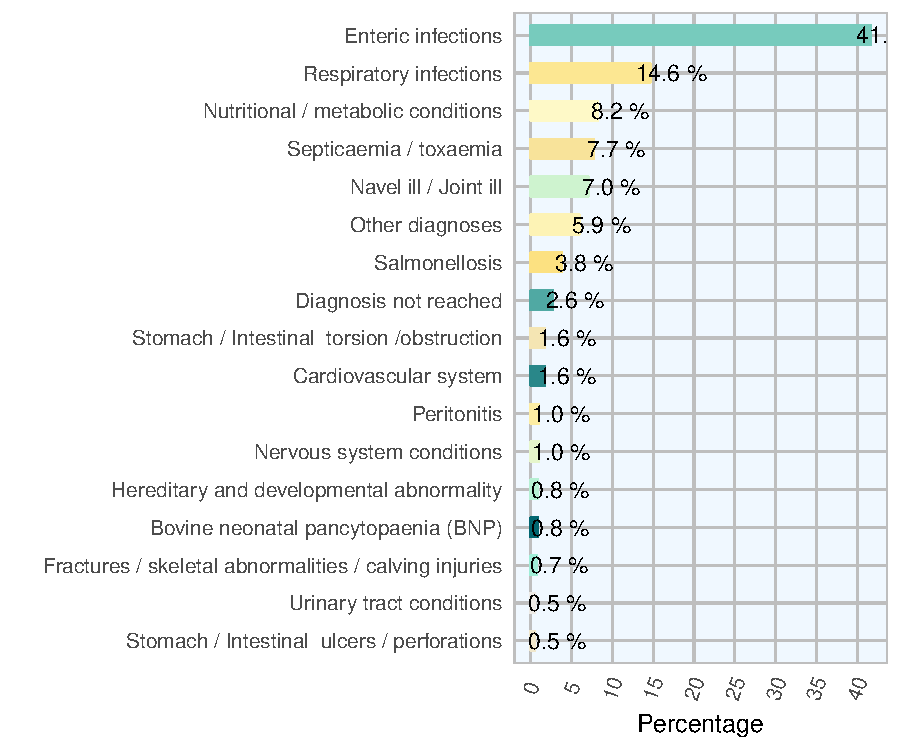
\includegraphics{AFBI_files/figure-latex/unnamed-chunk-7-1} 

}

\caption{The conditions most frequently diagnosed on post-mortem examinations of neonatal calves (0-1 months) by AFBI during 2017 (n= 610 )}\label{fig:unnamed-chunk-7}
\end{figure}

\section{Calves (1-5 months)}\label{calves-1-5-months}

\begin{table}

\caption{\label{tab:unnamed-chunk-10}The conditions most frequently diagnosed on *post-mortem* examinations of calves (1-5 months) in  AFBI during 2017  (n= 369 )}
\centering
\begin{tabular}[t]{l|r|r}
\hline
Category & Count & Percentage\\
\hline
Respiratory infections & 186 & 50.4\\
\hline
Enteric infections & 35 & 9.5\\
\hline
Diagnosis not reached & 19 & 5.2\\
\hline
Nutritional / metabolic conditions & 18 & 4.9\\
\hline
GIT torsions /obstruction & 17 & 4.6\\
\hline
Peritonitis & 15 & 4.1\\
\hline
Other diagnoses & 14 & 3.8\\
\hline
Septicaemia / toxaemia & 13 & 3.5\\
\hline
Clostridial disease & 11 & 3.0\\
\hline
Navel ill / Joint ill & 11 & 3.0\\
\hline
Cardiovascular conditions & 9 & 2.4\\
\hline
Urinary tract conditions & 6 & 1.6\\
\hline
CNS conditions & 6 & 1.6\\
\hline
GIT ulcer / perforation & 5 & 1.4\\
\hline
Poisoning & 2 & 0.5\\
\hline
BVD /Mucosal disease & 2 & 0.5\\
\hline
\end{tabular}
\end{table}

\begin{figure}

{\centering 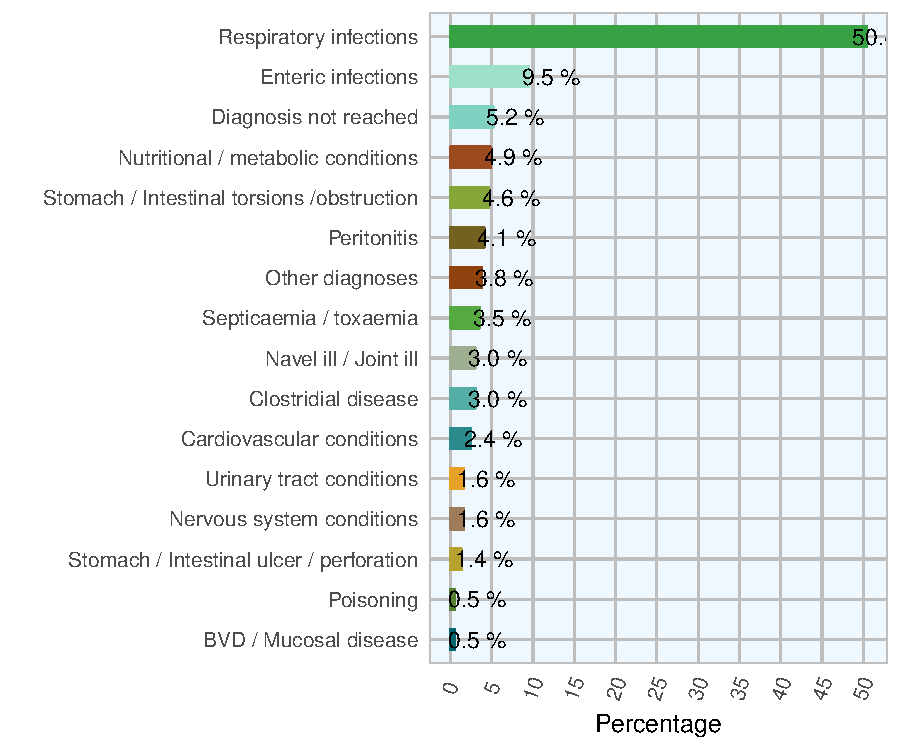
\includegraphics{AFBI_files/figure-latex/unnamed-chunk-11-1} 

}

\caption{The conditions most frequently diagnosed on *post-mortem* examinations of calves (1-5 months) by AFBI during 2017 (n= 369 )}\label{fig:unnamed-chunk-11}
\end{figure}

\section{Calves (6-12 months)}\label{calves-6-12-months}

\begin{table}

\caption{\label{tab:unnamed-chunk-13}The conditions most frequently diagnosed on *post-mortem* examinations of calves (6-12 months) in  AFBI during 2017 (n= 163 )}
\centering
\begin{tabular}[t]{l|r|r}
\hline
Category & Count & Percentage\\
\hline
Respiratory tract infections & 80 & 49.1\\
\hline
Clostridial disease & 18 & 11.0\\
\hline
Diagnosis not reached & 17 & 10.4\\
\hline
Nutritional / metabolic conditions & 11 & 6.8\\
\hline
Enteric infections & 8 & 4.9\\
\hline
Other diagnoses & 6 & 3.7\\
\hline
urinary tract conditions & 3 & 1.8\\
\hline
GIT ulcer, perforation, for body & 3 & 1.8\\
\hline
liver disease & 3 & 1.8\\
\hline
Poisoning & 3 & 1.8\\
\hline
GIT torsion / obstruction & 2 & 1.2\\
\hline
Cardiac conditions & 2 & 1.2\\
\hline
BVD / Mucosal disease & 2 & 1.2\\
\hline
CNS conditions & 2 & 1.2\\
\hline
Skeletal conditions & 2 & 1.2\\
\hline
peritonitis & 1 & 0.6\\
\hline
\end{tabular}
\end{table}

\begin{figure}

{\centering 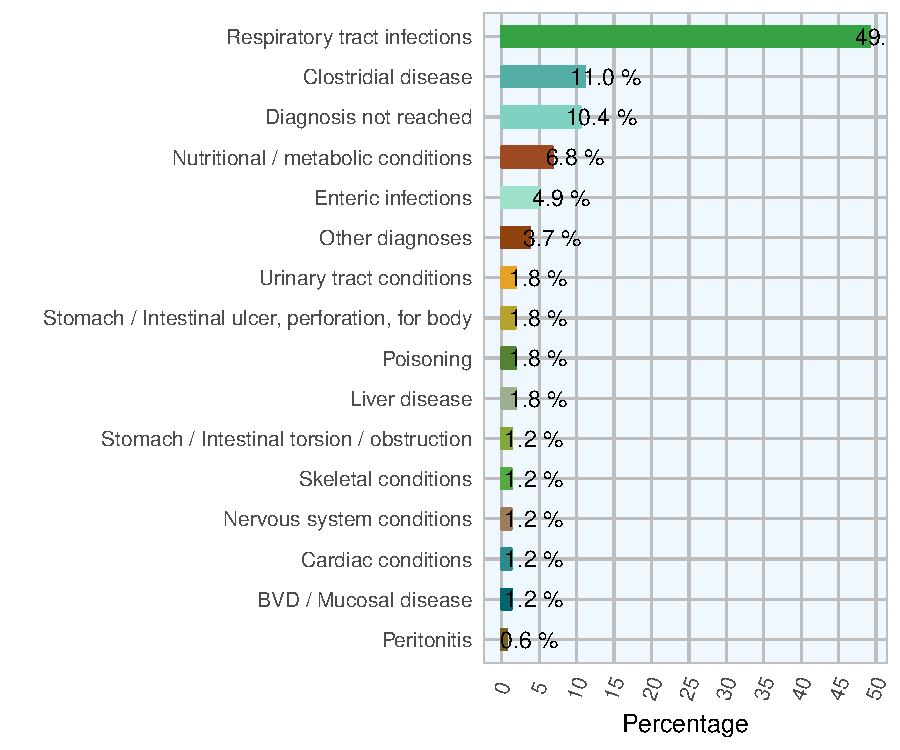
\includegraphics{AFBI_files/figure-latex/unnamed-chunk-14-1} 

}

\caption{The conditions most frequently diagnosed on *post-mortem* examinations of  calves (6-12 months) by AFBI during 2017 (n= 163 )}\label{fig:unnamed-chunk-14}
\end{figure}

\section{Adults (\textgreater{} 12 months)}\label{adults-12-months}

\begin{table}

\caption{\label{tab:unnamed-chunk-16}The conditions most frequently diagnosed on *post-mortem* examinations of adults (>12 months) by AFBI during 2017 (n= 464 )}
\centering
\begin{tabular}[t]{l|r|r}
\hline
Category & Count & Percentage\\
\hline
Respiratory infections & 95 & 20.5\\
\hline
Other diagnoses & 56 & 12.1\\
\hline
Diagnosis not reached & 55 & 11.8\\
\hline
Cardiac/ circulatory system & 50 & 10.8\\
\hline
Clostridial disease & 39 & 8.4\\
\hline
Nutritional /metabolic conditions & 36 & 7.8\\
\hline
Liver disease & 29 & 6.2\\
\hline
GIT ulceration / perforation / foreign body & 24 & 5.2\\
\hline
Enteric infections & 19 & 4.1\\
\hline
Reproductive tract infections/Mastitis & 12 & 2.6\\
\hline
Intestinal or gastric torsion /obstruction & 10 & 2.2\\
\hline
Peritonitis & 10 & 2.2\\
\hline
Urinary tract conditions & 9 & 1.9\\
\hline
Poisoning & 9 & 1.9\\
\hline
Tumour & 6 & 1.3\\
\hline
CNS infections & 5 & 1.1\\
\hline
\end{tabular}
\end{table}

\begin{figure}

{\centering 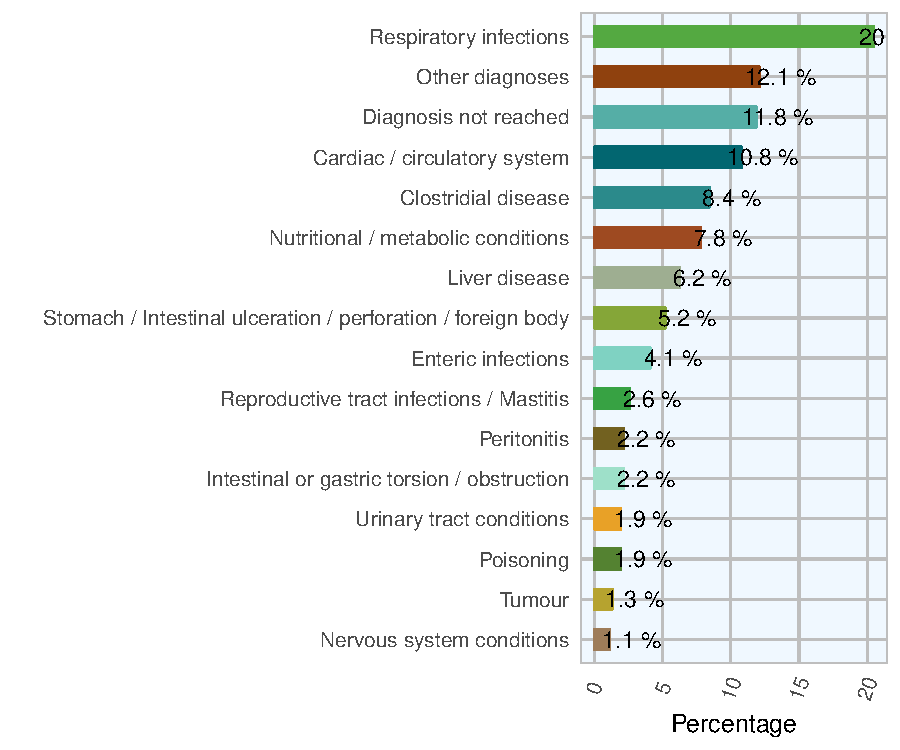
\includegraphics{AFBI_files/figure-latex/unnamed-chunk-17-1} 

}

\caption{The conditions most frequently diagnosed on *post-mortem* examinations of  adults (>12 months) by AFBI during 2017, (n= 464 )}\label{fig:unnamed-chunk-17}
\end{figure}

\chapter{Ovine Diseases}\label{ovine-diseases}

\begin{center}\rule{0.5\linewidth}{\linethickness}\end{center}

\begin{table}

\caption{\label{tab:unnamed-chunk-21}The most commom diagnosic groups on *post-mortem* examinations of ovine by AFBI in 2017 (n= 559 )}
\centering
\begin{tabular}[t]{l|r|r}
\hline
Category & Count & Percentage\\
\hline
Parasitic Disease & 188 & 33.6\\
\hline
Enteritis & 158 & 28.3\\
\hline
Respiratory Disease & 73 & 13.1\\
\hline
Septicemia & 36 & 6.4\\
\hline
Clostridial diseases & 32 & 5.7\\
\hline
CNS & 27 & 4.8\\
\hline
Metabolic & 23 & 4.1\\
\hline
Poisoning & 22 & 3.9\\
\hline
\end{tabular}
\end{table}

\begin{figure}

{\centering 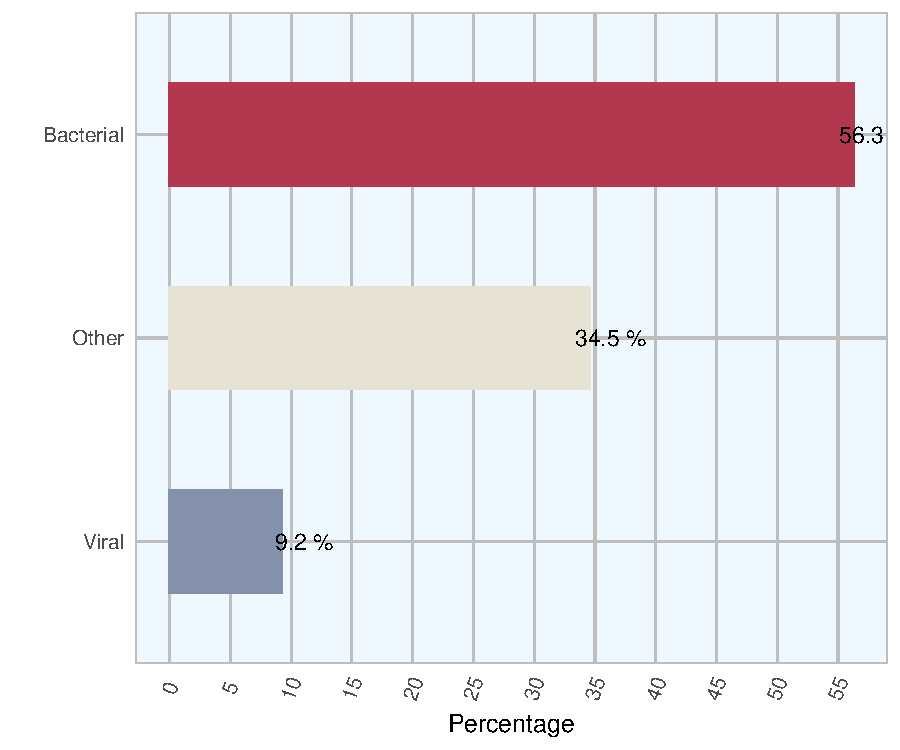
\includegraphics{AFBI_files/figure-latex/unnamed-chunk-22-1} 

}

\caption{The conditions most frequently diagnosed on *post-mortem* examinations of  ovine carcasses in 2017(n= 559 )}\label{fig:unnamed-chunk-22}
\end{figure}

\begin{table}

\caption{\label{tab:unnamed-chunk-24}The frequency of the most commom diagnosic group on *post-mortem* examinations of ovine carcasses by during 2017 (n= 559 )}
\centering
\begin{tabular}[t]{l|l|r|r|r}
\hline
Category & Disease & Count & Pct within group & Pct\\
\hline
Septicemia & Pasteurella septicaemia & 18 & 50.0 & 3.2\\
\hline
Septicemia & Colisepticaemia & 9 & 25.0 & 1.6\\
\hline
Septicemia & Septicaemia NOS & 5 & 13.9 & 0.9\\
\hline
Septicemia & Systemic pasteurellosis & 3 & 8.3 & 0.5\\
\hline
Septicemia & Navel-ill / joint-ill & 1 & 2.8 & 0.2\\
\hline
Respiratory Disease & Pulmonia Adenomatosis - Jaagsiekte & 29 & 39.7 & 5.2\\
\hline
Respiratory Disease & P Haemolytica & 18 & 24.7 & 3.2\\
\hline
Respiratory Disease & Pneumonis Nos & 10 & 13.7 & 1.8\\
\hline
Respiratory Disease & Parasitic pneumonia & 6 & 8.2 & 1.1\\
\hline
Respiratory Disease & Bronchopneumonia & 3 & 4.1 & 0.5\\
\hline
Respiratory Disease & Laryngael Chondritis & 3 & 4.1 & 0.5\\
\hline
Respiratory Disease & Fibrinous Pleurisy & 2 & 2.7 & 0.4\\
\hline
Respiratory Disease & Necrotising Laryngitis & 1 & 1.4 & 0.2\\
\hline
Respiratory Disease & Viral Pneumonia & 1 & 1.4 & 0.2\\
\hline
Poisoning & Poisoning DT pieris & 14 & 63.6 & 2.5\\
\hline
Poisoning & Poisoning DT copper & 4 & 18.2 & 0.7\\
\hline
Poisoning & Poisoning DT plant NOS & 2 & 9.1 & 0.4\\
\hline
Poisoning & Poisoning DT rhododendron & 2 & 9.1 & 0.4\\
\hline
Parasitic Disease & PGE Nos & 69 & 36.7 & 12.3\\
\hline
Parasitic Disease & Chronic Fascioliasis & 50 & 26.6 & 8.9\\
\hline
Parasitic Disease & Coccidiosis & 24 & 12.8 & 4.3\\
\hline
Parasitic Disease & PGE- Nematodiriasis & 24 & 12.8 & 4.3\\
\hline
Parasitic Disease & Acute Fascioliasis & 21 & 11.2 & 3.8\\
\hline
Metabolic & Acidosis & 10 & 43.5 & 1.8\\
\hline
Metabolic & Twin lamb disease & 7 & 30.4 & 1.2\\
\hline
Metabolic & Hypocalcaemia & 3 & 13.0 & 0.5\\
\hline
Metabolic & Pregnancy toxaemia & 2 & 8.7 & 0.4\\
\hline
Metabolic & Hypomagnesaemia & 1 & 4.3 & 0.2\\
\hline
Enteritis & PGE – NOS & 69 & 43.7 & 12.3\\
\hline
Enteritis & Coccidiosis & 24 & 15.2 & 4.3\\
\hline
Enteritis & PGE – nematodiriasis & 24 & 15.2 & 4.3\\
\hline
Enteritis & Diarrhoea NOS & 10 & 6.3 & 1.8\\
\hline
Enteritis & Enteritis NOS & 8 & 5.1 & 1.4\\
\hline
Enteritis & Abomasitis & 6 & 3.8 & 1.1\\
\hline
Enteritis & Colibacillosis – enteric & 3 & 1.9 & 0.5\\
\hline
Enteritis & Colienteritis & 3 & 1.9 & 0.5\\
\hline
Enteritis & Cryptosporidiosis & 2 & 1.3 & 0.4\\
\hline
Enteritis & Johne’s disease & 2 & 1.3 & 0.4\\
\hline
Enteritis & Perforated intestine & 2 & 1.3 & 0.4\\
\hline
Enteritis & Watery mouth & 2 & 1.3 & 0.4\\
\hline
Enteritis & Colibacillosis enteric – K99 positive & 1 & 0.6 & 0.2\\
\hline
Enteritis & Red gut & 1 & 0.6 & 0.2\\
\hline
Enteritis & Tapeworm infestation & 1 & 0.6 & 0.2\\
\hline
CNS & Encephalitis DT Listeria sp & 11 & 40.7 & 2.0\\
\hline
CNS & Meningitis / encephalitis & 6 & 22.2 & 1.1\\
\hline
CNS & Listeriosis & 4 & 14.8 & 0.7\\
\hline
CNS & Cerebrocortical necrosis & 3 & 11.1 & 0.5\\
\hline
CNS & Encephalitis NOS & 2 & 7.4 & 0.4\\
\hline
CNS & Brain hemorrhage & 1 & 3.7 & 0.2\\
\hline
Clostridial diseases & Pulpy kidney diseases & 12 & 37.5 & 2.1\\
\hline
Clostridial diseases & Pulpy kidney & 11 & 34.4 & 2.0\\
\hline
Clostridial diseases & Black disease & 4 & 12.5 & 0.7\\
\hline
Clostridial diseases & Clost Dis NOS & 3 & 9.4 & 0.5\\
\hline
Clostridial diseases & Enterotoxaemia & 2 & 6.2 & 0.4\\
\hline
\end{tabular}
\end{table}

\section{Diagnoses by Group}\label{diagnoses-by-group}

\subsection{Septicaemia}\label{septicaemia}

\begin{figure}

{\centering 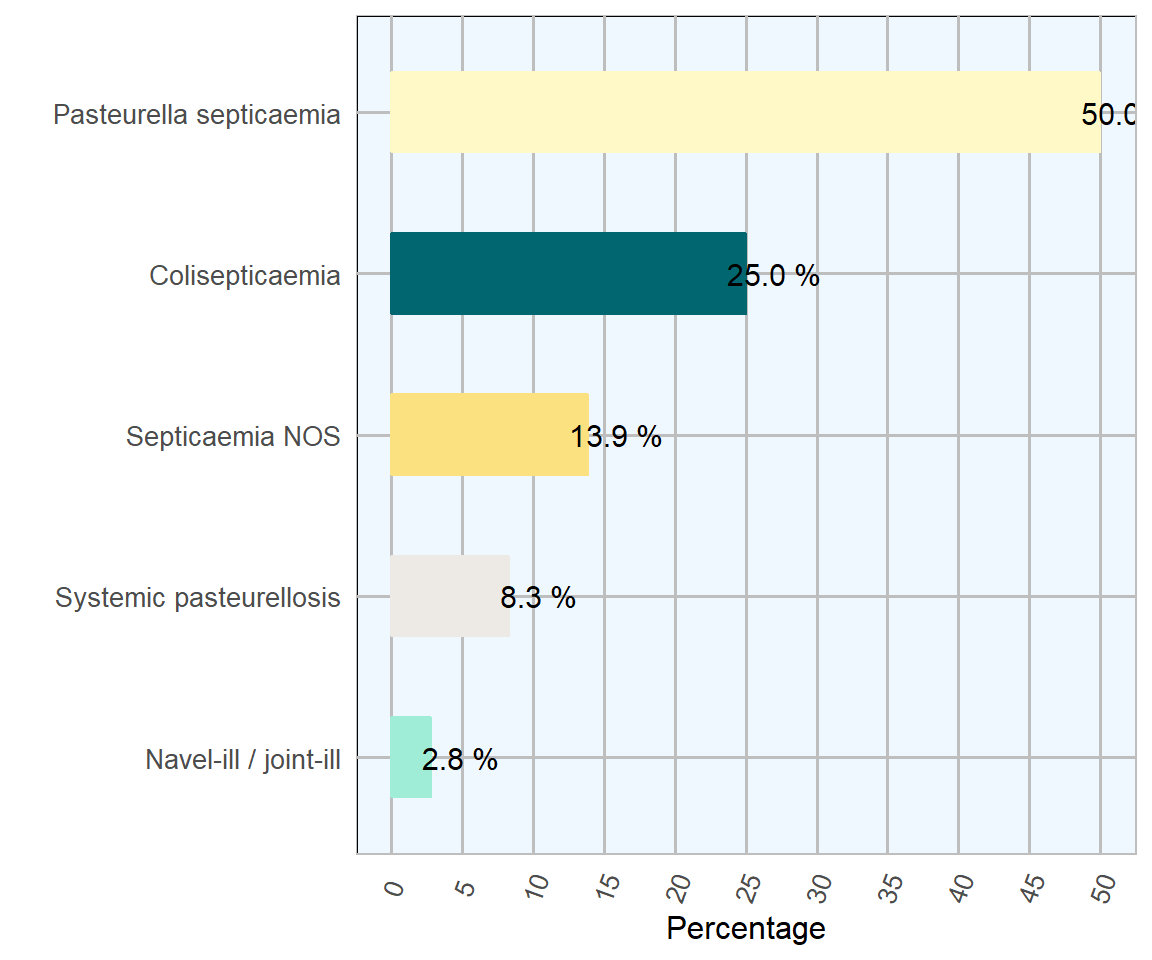
\includegraphics{AFBI_files/figure-latex/unnamed-chunk-26-1} 

}

\caption{The septicaemic conditions most frequently diagnosed on post-mortem examinations of ovine by AFBI during 2017(n= 36 )}\label{fig:unnamed-chunk-26}
\end{figure}

\subsection{Respiratory Disease}\label{respiratory-disease}

\begin{figure}

{\centering 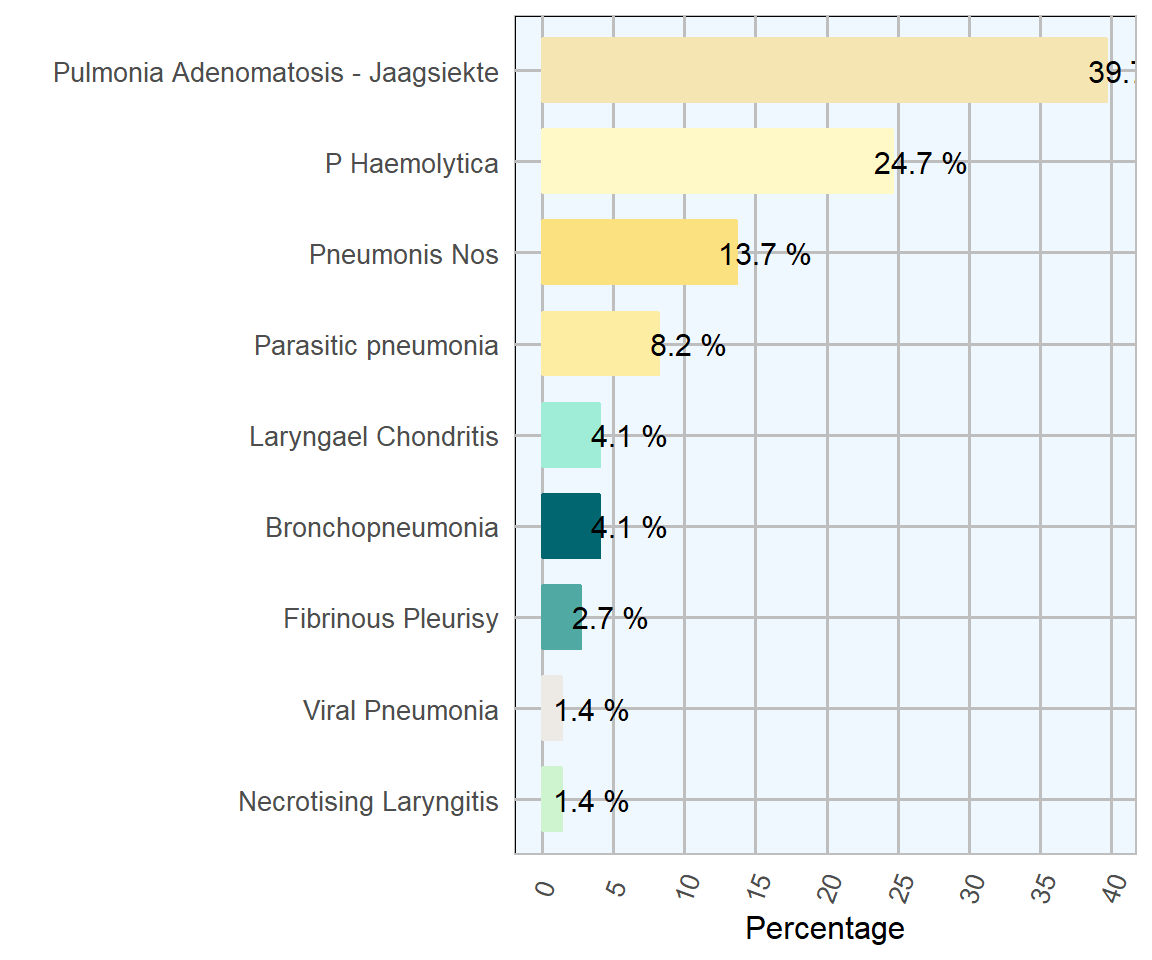
\includegraphics{AFBI_files/figure-latex/unnamed-chunk-28-1} 

}

\caption{The respiratory conditions most frequently diagnosed on post-mortem examinations of ovine by AFBI during 2017 (n= 73 )}\label{fig:unnamed-chunk-28}
\end{figure}

\subsection{Poisoning}\label{poisoning}

\begin{figure}

{\centering 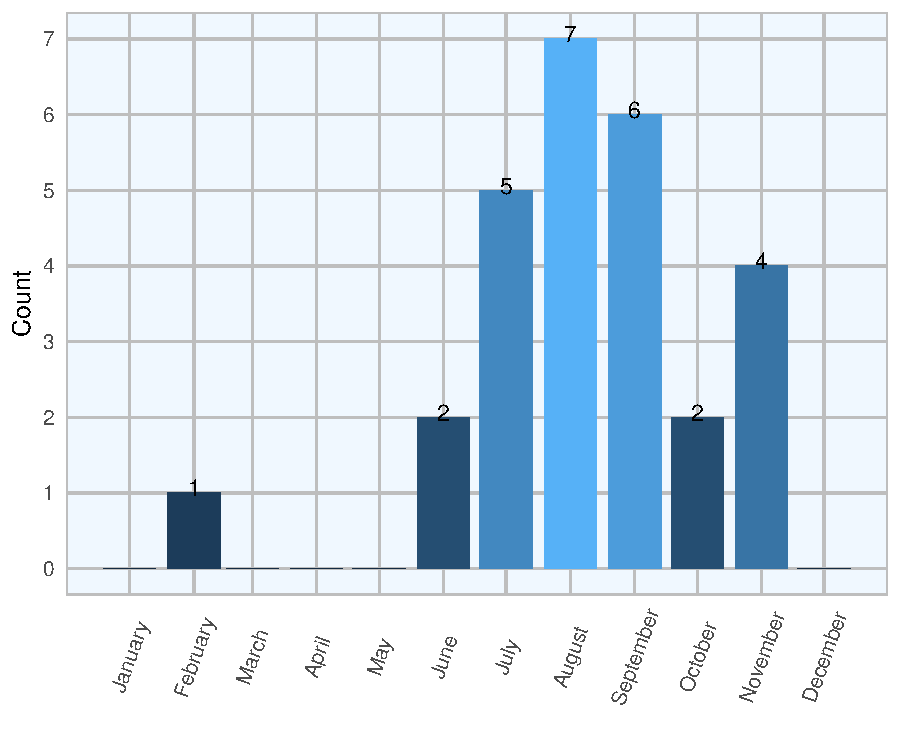
\includegraphics{AFBI_files/figure-latex/unnamed-chunk-30-1} 

}

\caption{The poisoning agents most frequently diagnosed on post-mortem examinations of ovine  by AFBI during 2017 (n= 22 )}\label{fig:unnamed-chunk-30}
\end{figure}

\subsection{Parasitic Disease}\label{parasitic-disease}

\begin{figure}

{\centering 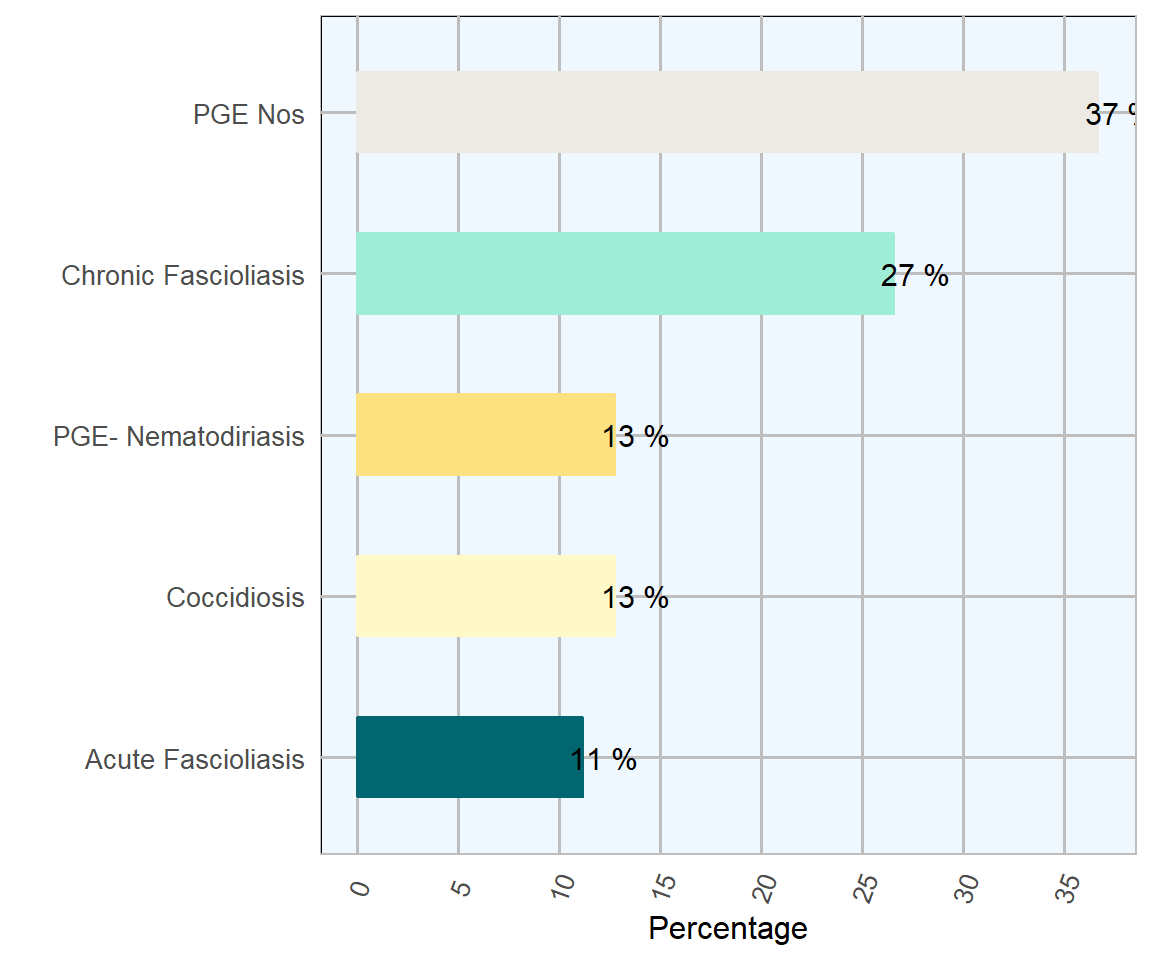
\includegraphics{AFBI_files/figure-latex/unnamed-chunk-32-1} 

}

\caption{The parasitic conditions most frequently diagnosed on post-mortem examinations of ovine by AFBI during 2017 (n= 188 )}\label{fig:unnamed-chunk-32}
\end{figure}

\subsection{Metabolic}\label{metabolic}

\begin{figure}

{\centering 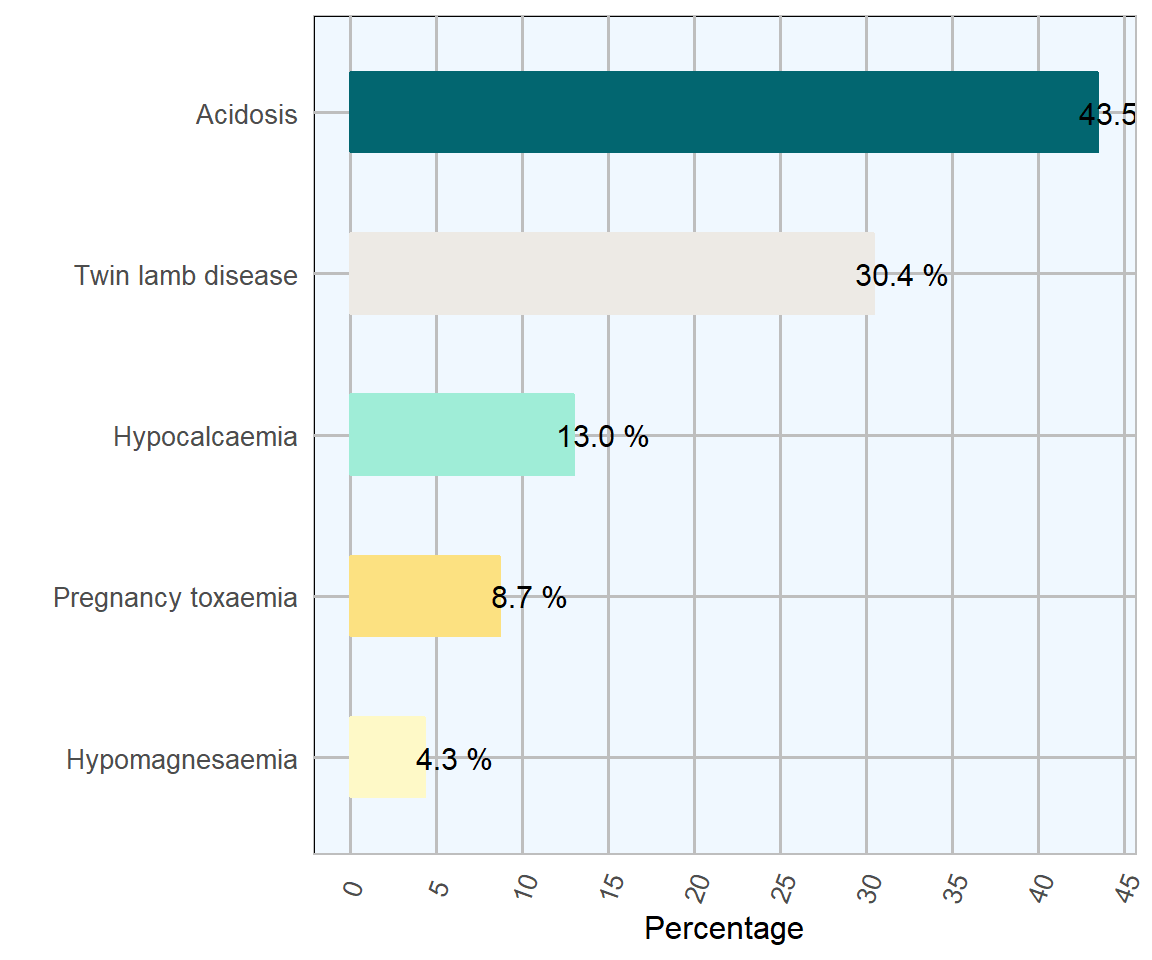
\includegraphics{AFBI_files/figure-latex/unnamed-chunk-34-1} 

}

\caption{The metabolic conditions most frequently diagnosed on post-mortem examinations of ovine by AFBI during 2017(n= 23 )}\label{fig:unnamed-chunk-34}
\end{figure}

\subsection{Enteritis}\label{enteritis}

\begin{figure}

{\centering 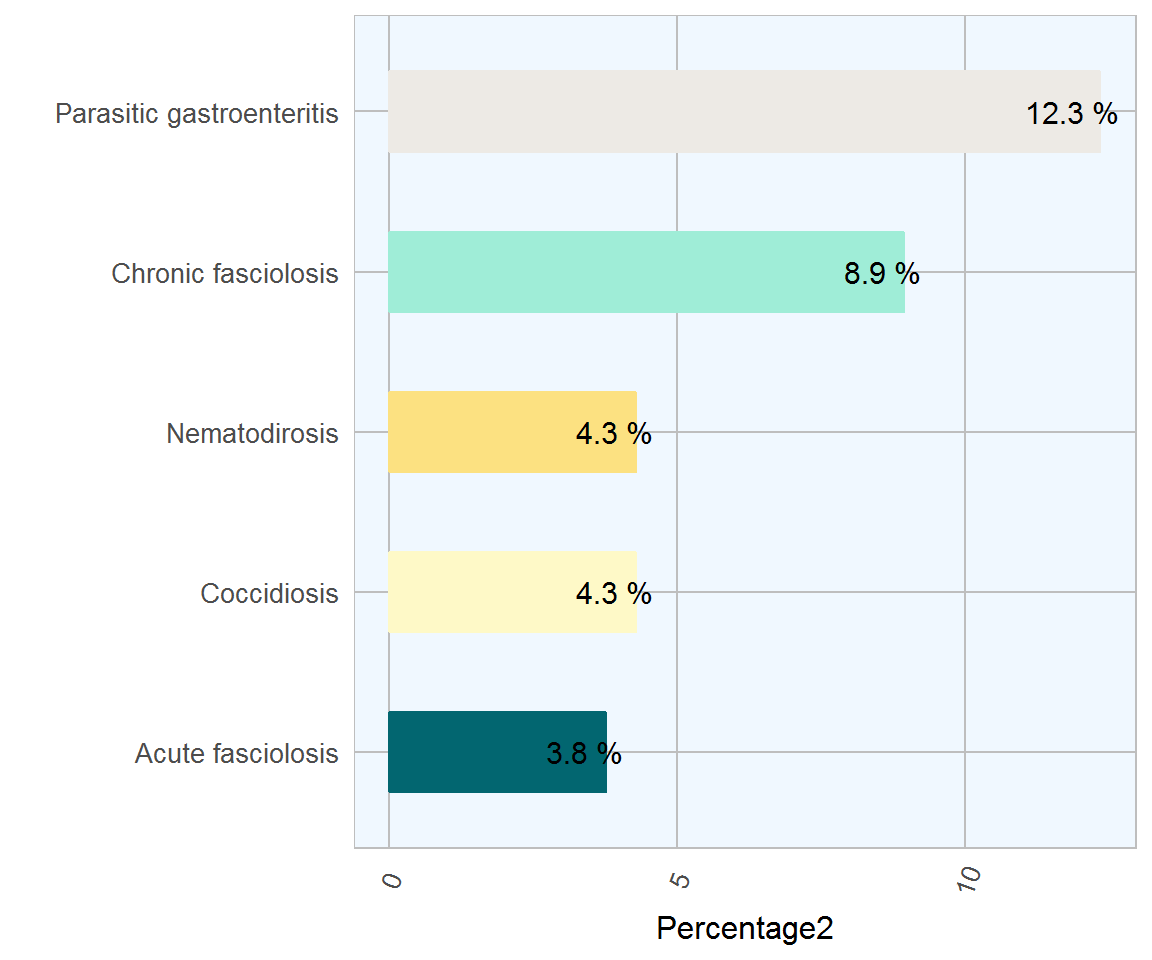
\includegraphics{AFBI_files/figure-latex/unnamed-chunk-36-1} 

}

\caption{The enteric conditions most frequently diagnosed on post-mortem examinations of ovine by AFBI during 2017 (n= 158 )}\label{fig:unnamed-chunk-36}
\end{figure}

\subsection{CNS}\label{cns}

\begin{figure}

{\centering 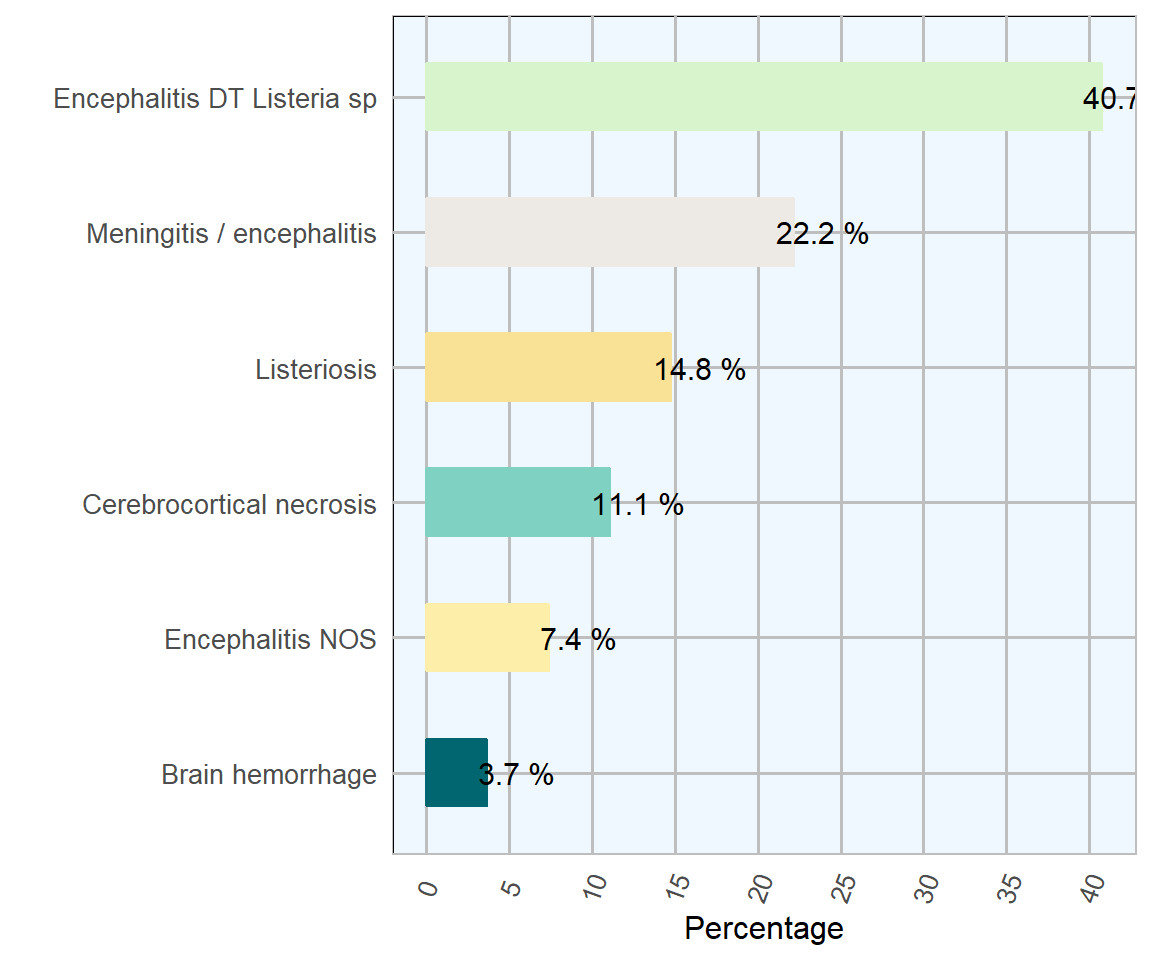
\includegraphics{AFBI_files/figure-latex/unnamed-chunk-38-1} 

}

\caption{The CND conditions most frequently diagnosed on post-mortem examinations of ovine by AFBI during 2017 (n= 27 )}\label{fig:unnamed-chunk-38}
\end{figure}

\subsection{Clostridial diseases}\label{clostridial-diseases}

\begin{figure}

{\centering 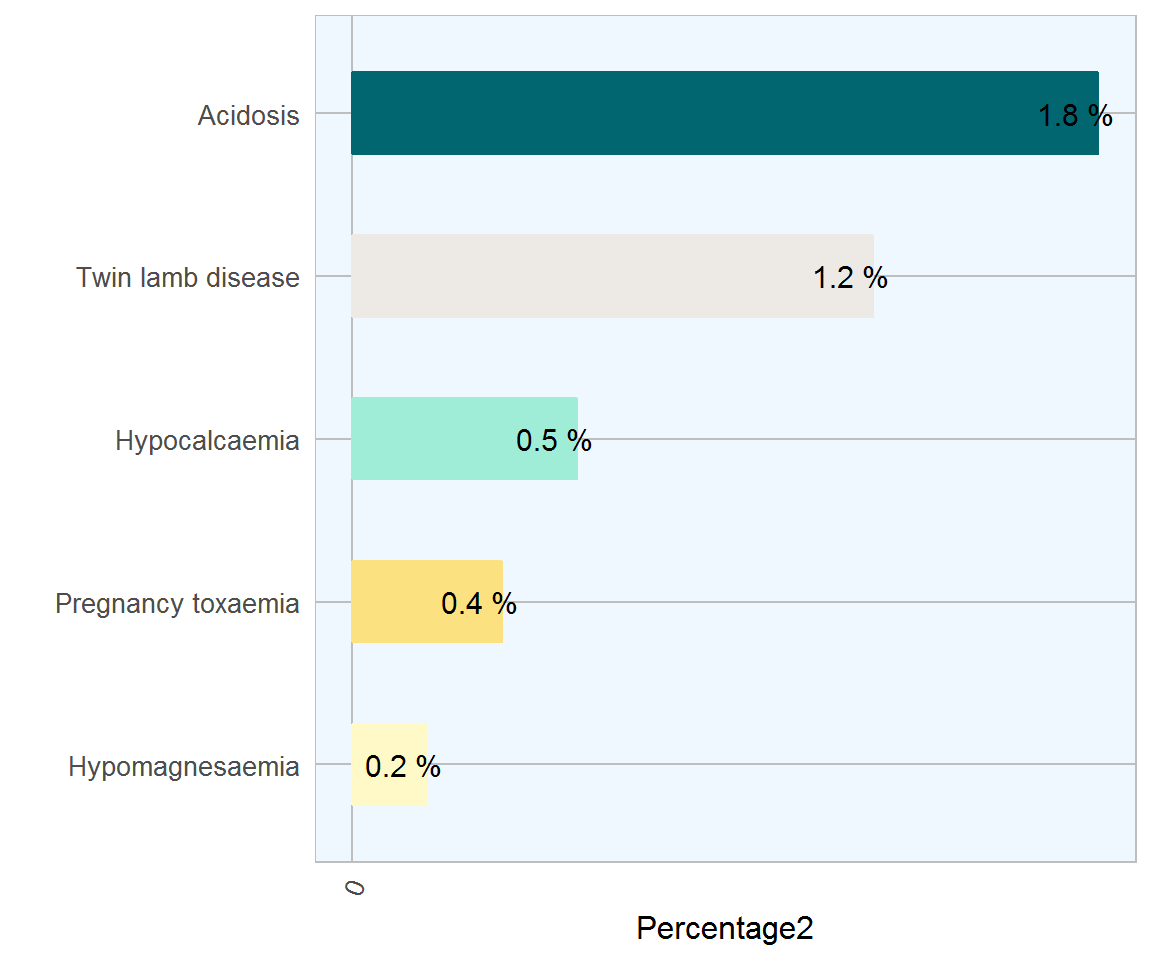
\includegraphics{AFBI_files/figure-latex/unnamed-chunk-40-1} 

}

\caption{The clostridial diseases most frequently diagnosed on post-mortem examinations of ovine by AFBI during 2017(n= 32 )}\label{fig:unnamed-chunk-40}
\end{figure}

\chapter{Bovine Respiratory Disease
(BRD)}\label{bovine-respiratory-disease-brd}

\begin{center}\rule{0.5\linewidth}{\linethickness}\end{center}

\section{Diagnoses by Group}\label{diagnoses-by-group-1}

\begin{table}

\caption{\label{tab:unnamed-chunk-44}The most commom diagnosic groups on *post-mortem* examinations of bovine respiratory disease by AFBI during 2017 (n= 391 )}
\centering
\begin{tabular}[t]{l|r|r}
\hline
Category & Count & Percentage\\
\hline
Bacterial & 220 & 56.3\\
\hline
Miscellaneous & 135 & 34.5\\
\hline
Viral & 36 & 9.2\\
\hline
\end{tabular}
\end{table}

\begin{figure}

{\centering 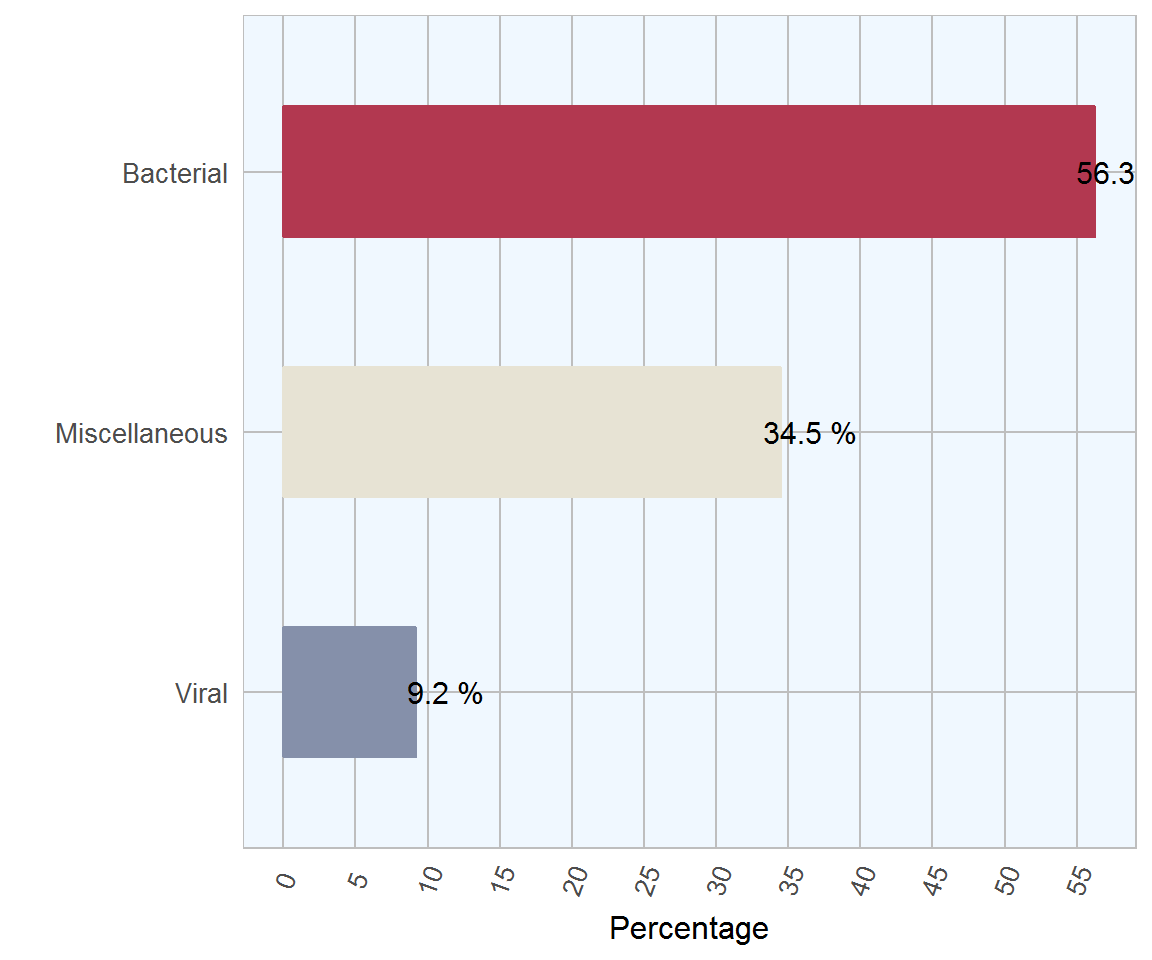
\includegraphics{AFBI_files/figure-latex/unnamed-chunk-45-1} 

}

\caption{The most commom diagnosic groups on *post-mortem* examinations of bovine respiratory disease by AFBI during 2017 (n= 391 )}\label{fig:unnamed-chunk-45}
\end{figure}

\subsection{Bovine Respiratory Disease
Diagnoses}\label{bovine-respiratory-disease-diagnoses}

\begin{table}

\caption{\label{tab:unnamed-chunk-49}Relative frequency of diagnoses in bovine respiratory disease recorded by AFBI during 2017, (n= 391 )}
\centering
\begin{tabular}[t]{l|r|r}
\hline
Category & Count & Percentage\\
\hline
PNEUMONIA DT MYCOPLASMA BOVIS & 90 & 23.0\\
\hline
PNEUMONIA NOS & 70 & 17.9\\
\hline
PNEUMONIA DT P MULTOCIDA & 45 & 11.5\\
\hline
PNEUMONIA A PYOGENES & 35 & 8.9\\
\hline
PNEUMONIA DT M HAEMOLYTICA & 33 & 8.4\\
\hline
PNEUMONIA - PARASITIC - HUSK & 27 & 6.9\\
\hline
PNEUMONIA - RSV & 15 & 3.8\\
\hline
FIBRINOUS PLEURISY & 14 & 3.6\\
\hline
IBR & 12 & 3.1\\
\hline
PNEUMONIA - H SOMNUS & 10 & 2.6\\
\hline
CHRONIC BRONCHOPNEUMONIA & 6 & 1.5\\
\hline
PNEUMONIA - BVD & 5 & 1.3\\
\hline
PNEUMONIA DT ASPIRATION & 4 & 1.0\\
\hline
SEVERE TRACHEITIS & 4 & 1.0\\
\hline
FRACTURED RIBS & 3 & 0.8\\
\hline
PASTEURELLOSIS & 3 & 0.8\\
\hline
MALIGNANT CATARRH & 2 & 0.5\\
\hline
PNEUMONIA - FUNGAL & 2 & 0.5\\
\hline
PNEUMONIA - P13 & 2 & 0.5\\
\hline
PNEUMONIA DT ACTINO & 2 & 0.5\\
\hline
PULMONARY EMBOLISM & 2 & 0.5\\
\hline
TUBERCULOSIS & 2 & 0.5\\
\hline
ADENOCARCINOMA & 1 & 0.3\\
\hline
ATELECTASIS & 1 & 0.3\\
\hline
PULMONARYHAEMORRHAGE & 1 & 0.3\\
\hline
\end{tabular}
\end{table}

\begin{figure}

{\centering 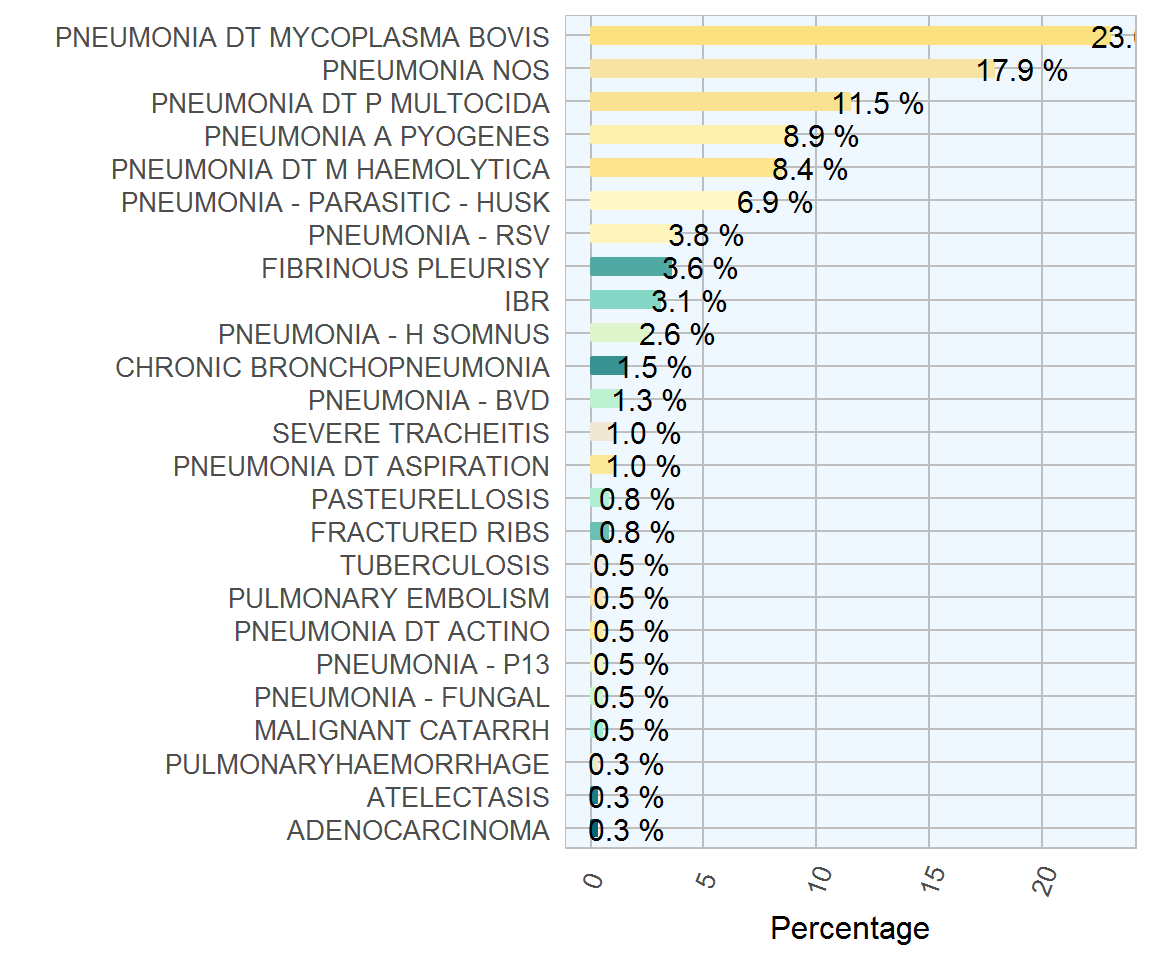
\includegraphics{AFBI_files/figure-latex/unnamed-chunk-50-1} 

}

\caption{Relative frequency of diagnoses in bovine respiratory disease recorded by AFBI during 2017, (n= 391 )}\label{fig:unnamed-chunk-50}
\end{figure}

\subsection{Lungworm}\label{lungworm}

\begin{figure}

{\centering 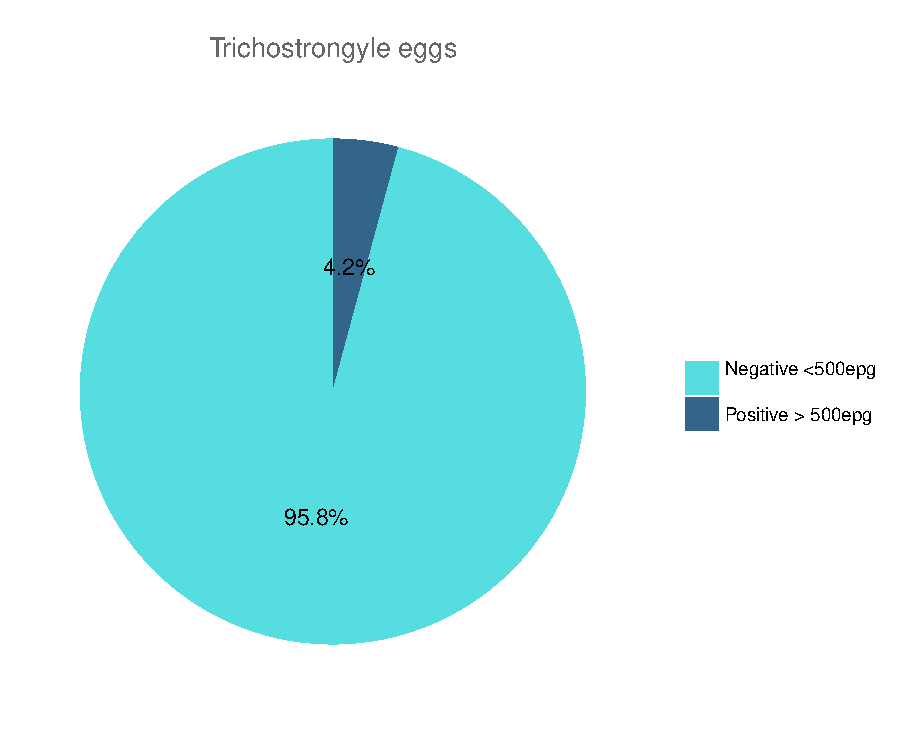
\includegraphics{AFBI_files/figure-latex/unnamed-chunk-53-1} 

}

\caption{Evolution of the number of lungworm  respiratory disease recorded by AFBI during 2017, (n= 27 )}\label{fig:unnamed-chunk-53}
\end{figure}

\chapter{Bovine Abortions}\label{bovine-abortions}

\begin{center}\rule{0.5\linewidth}{\linethickness}\end{center}

\begin{table}

\caption{\label{tab:unnamed-chunk-57}The frequently of the most commom diagnoses in bovine abortion in  AFBI during 2017 (n= 427 )}
\centering
\begin{tabular}[t]{l|r|r}
\hline
Category & Count & Percentage\\
\hline
Undiagnosed & 229 & 53.6\\
\hline
T. pyogenes & 37 & 8.7\\
\hline
B. licheniformis & 35 & 8.2\\
\hline
N. caninum & 21 & 4.9\\
\hline
BVDV & 15 & 3.5\\
\hline
E. coli & 15 & 3.5\\
\hline
S. dublin & 15 & 3.5\\
\hline
Leptospirosis & 12 & 2.8\\
\hline
Other & 12 & 2.8\\
\hline
Pasteurellosis & 9 & 2.1\\
\hline
Foetal abnormalities & 8 & 1.9\\
\hline
Schmallenberg Virus & 5 & 1.2\\
\hline
Mummification & 5 & 1.2\\
\hline
Listeria & 4 & 0.9\\
\hline
Campylobacter sp & 3 & 0.7\\
\hline
Aspergillosis & 2 & 0.5\\
\hline
\end{tabular}
\end{table}

\begin{figure}

{\centering 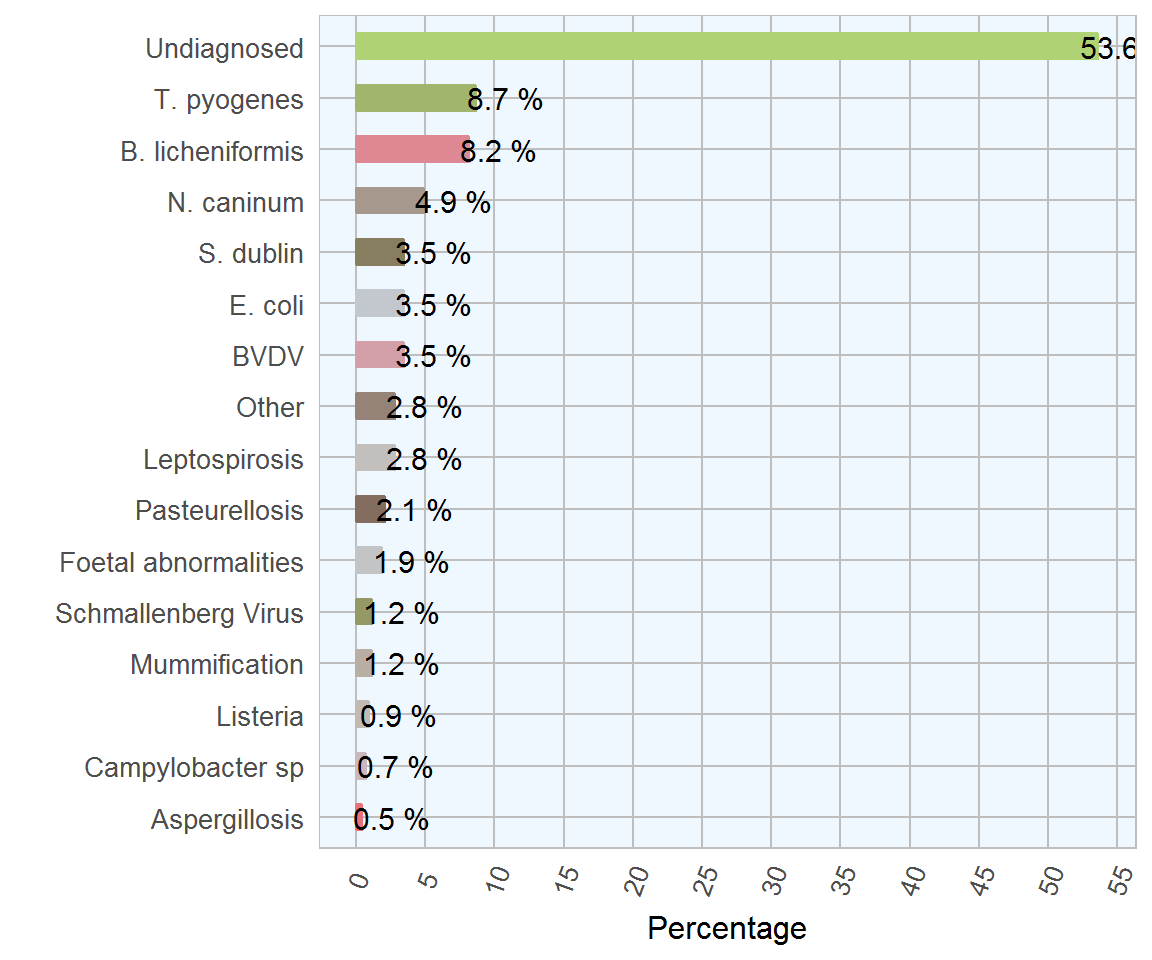
\includegraphics{AFBI_files/figure-latex/unnamed-chunk-58-1} 

}

\caption{The conditions most frequently diagnosed on post-mortem examinations of  ovine carcasses by AFBI during 2017 (n= 427 )}\label{fig:unnamed-chunk-58}
\end{figure}

\chapter{Ovine Abortions}\label{ovine-abortions}

\begin{table}

\caption{\label{tab:unnamed-chunk-62}The frequently of the most commom diagnosic group on *post-mortem* examinations ovine by AFBI during 2017}
\centering
\begin{tabular}[t]{l|r|r}
\hline
Category & Count & Percentage\\
\hline
Toxoplasma gondi & 74 & 30.3\\
\hline
No significant agent identified. & 67 & 27.5\\
\hline
Chlamydophilia abortus & 44 & 18.0\\
\hline
E.coli & 20 & 8.2\\
\hline
Campylobacter spp & 12 & 4.9\\
\hline
Streptococcus spp & 9 & 3.7\\
\hline
Leptospirosis & 8 & 3.3\\
\hline
Arcanobacter pyogenes & 5 & 2.0\\
\hline
Listeria monocytogenes & 5 & 2.0\\
\hline
\end{tabular}
\end{table}

\begin{figure}

{\centering 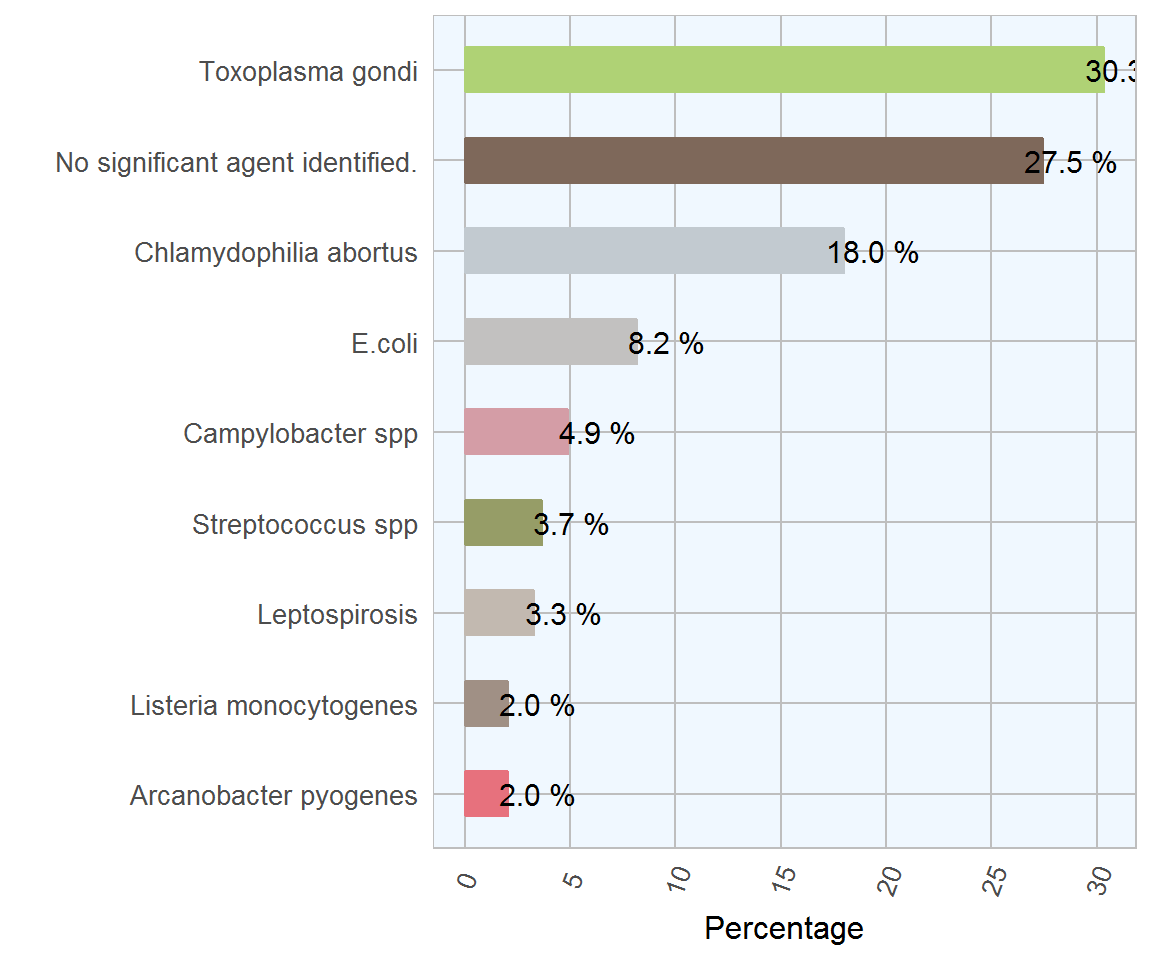
\includegraphics{AFBI_files/figure-latex/unnamed-chunk-63-1} 

}

\caption{The conditions most frequently diagnosed on post-mortem examinations of  ovine carcasses by AFBI during 2017}\label{fig:unnamed-chunk-63}
\end{figure}

\chapter{Bovine Mastitis}\label{bovine-mastitis}

\begin{center}\rule{0.5\linewidth}{\linethickness}\end{center}

\begin{table}

\caption{\label{tab:unnamed-chunk-67}hkdhkd in 2017}
\centering
\begin{tabular}[t]{l|r|r}
\hline
Microorganism & Count & Pct of Total\\
\hline
E.coli & 261 & 22.8\\
\hline
Streptococcus uberis & 156 & 13.6\\
\hline
Staphlococcus aureus & 97 & 8.5\\
\hline
Strep dysgalactiae & 28 & 2.4\\
\hline
Contaminated samples & 110 & 9.6\\
\hline
No bacteria cultured & 143 & 12.5\\
\hline
Other & 352 & 30.7\\
\hline
\end{tabular}
\end{table}

\begin{figure}

{\centering 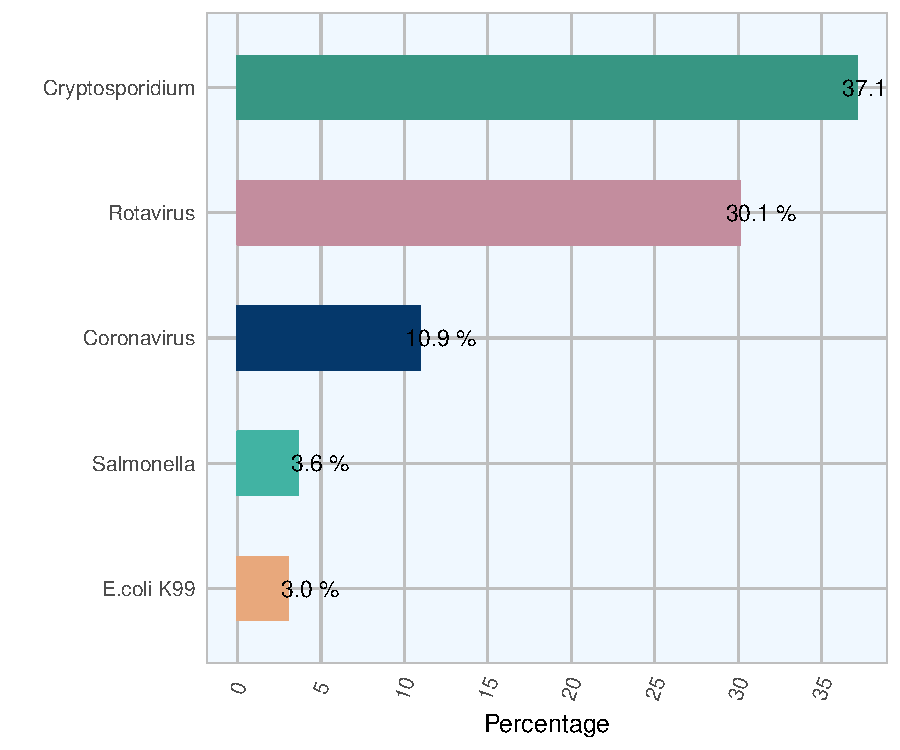
\includegraphics{AFBI_files/figure-latex/unnamed-chunk-68-1} 

}

\caption{Relative frequency of detection of selected mastitis pathogens by AFBI}\label{fig:unnamed-chunk-68}
\end{figure}

\chapter{Bovine Parasites}\label{bovine-parasites}

\begin{center}\rule{0.5\linewidth}{\linethickness}\end{center}

\begin{table}

\caption{\label{tab:unnamed-chunk-72}Count and percentage of positive results detected in bovine faecal samples examined by AFBI during 2017}
\centering
\begin{tabular}[t]{l|r|r|r}
\hline
Parasite & Negative & Positive & Pct of Positive\\
\hline
Coccidia & 2205 & 814 & 27.0\\
\hline
Fluke eggs & 2483 & 268 & 9.7\\
\hline
Nematodirus epg & 2984 & 36 & 1.2\\
\hline
Paramphistome eggs & 1266 & 1464 & 53.6\\
\hline
Strongyle epg & 2390 & 617 & 20.5\\
\hline
\end{tabular}
\end{table}

\begin{figure}

{\centering 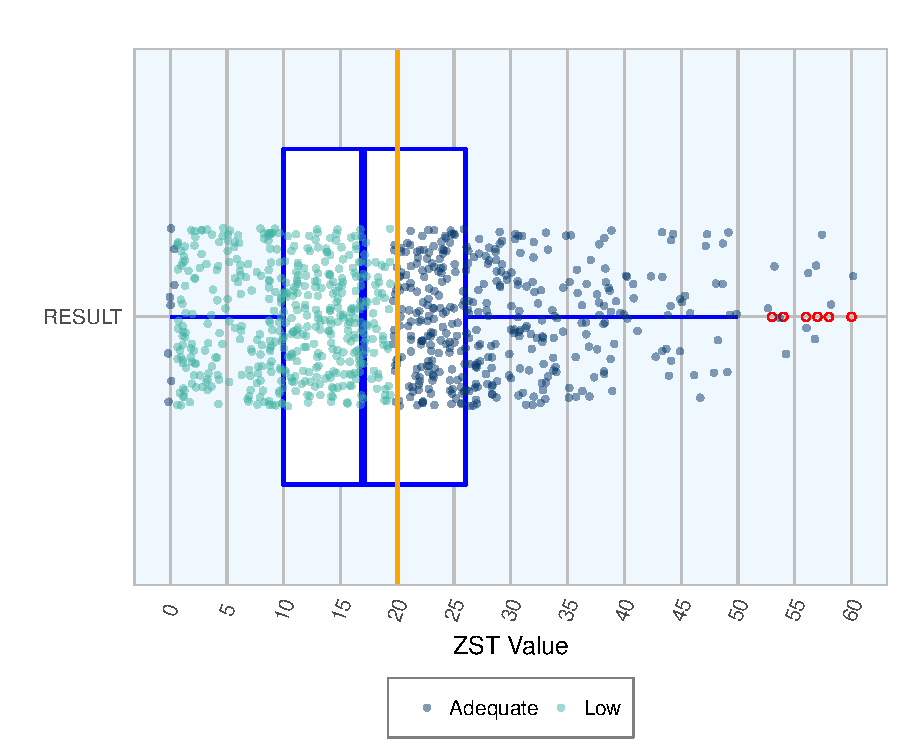
\includegraphics{AFBI_files/figure-latex/unnamed-chunk-74-1} 

}

\caption{Evolution of the number of positive results in bovine  samples in feacal submissions to AFBI during 2017}\label{fig:unnamed-chunk-74}
\end{figure}

\chapter{Ovine Parasites}\label{ovine-parasites}

\begin{center}\rule{0.5\linewidth}{\linethickness}\end{center}

\begin{table}

\caption{\label{tab:unnamed-chunk-78}Count  and percentage of positive results detected in ovine faecal samples examined by AFBI during 2017}
\centering
\begin{tabular}[t]{l|r|r|r}
\hline
Parasite & Negative & Positive & Pct of Positive\\
\hline
Coccidia & 533 & 1349 & 72\\
\hline
Fluke eggs & 1564 & 217 & 12\\
\hline
Nematodirus epg & 1635 & 278 & 14\\
\hline
Paramphistome eggs & 1219 & 561 & 32\\
\hline
Strongyle epg & 821 & 1065 & 56\\
\hline
\end{tabular}
\end{table}

\begin{figure}

{\centering 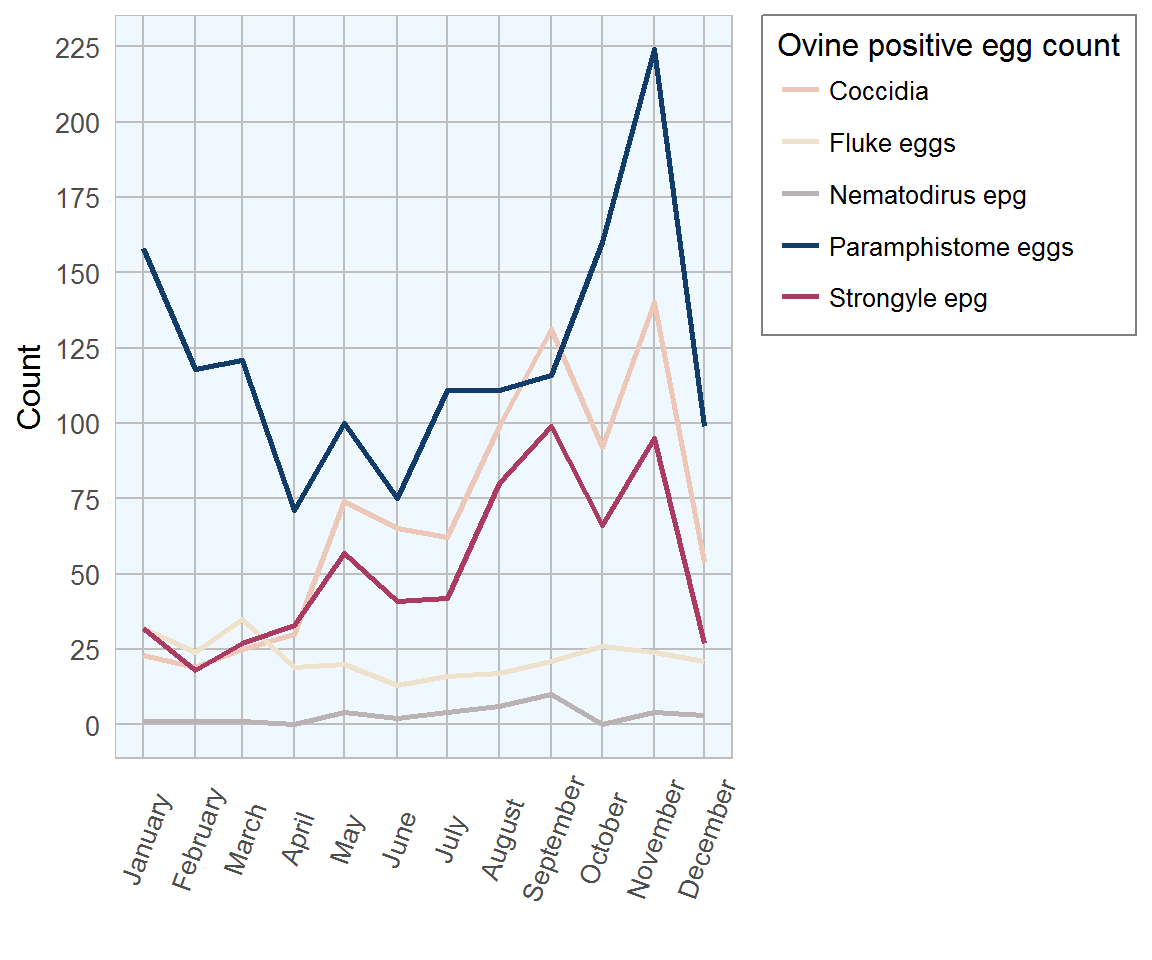
\includegraphics{AFBI_files/figure-latex/unnamed-chunk-80-1} 

}

\caption{Evolution of the number of positive results in ovine  samples in feacal submissions to AFBI during 2017}\label{fig:unnamed-chunk-80}
\end{figure}

\chapter{Zinc Sulphate Turbidity (ZST)
Test}\label{zinc-sulphate-turbidity-zst-test}

\begin{center}\rule{0.5\linewidth}{\linethickness}\end{center}

\begin{table}

\caption{\label{tab:unnamed-chunk-84}Zinc Sulphate Turbidity Test}
\centering
\begin{tabular}[t]{l|r|r|r|r|r}
\hline
Status & Count & Mean & Median & Minimum & Maximum\\
\hline
Adequate & 75 & 33 & 28 & 20 & 93\\
\hline
\end{tabular}
\end{table}

\bibliography{book.bib,packages.bib}


\end{document}
